\documentclass[a4paper,10pt]{article}
\usepackage[utf8]{inputenc}
\usepackage{graphicx}
%opening
\title{Offensive Security\\
	Lab-report
}
\author{Moritz Rupp}
\begin{document}

\maketitle
\tableofcontents
\begin{abstract}
Lab3 documentation
\end{abstract}
\newpage
\section{Exercise 3}
\subsection{UART Communication Analysis}
Salea offers an extension 'Saleae-Hex-Dec-Char-to-Terminal` that is capable of converting low level analyser output to human readable data. This way we can write the bewished encoding like ascii to a file of choice.\\
With the help of a simple Python script, it's now possible to read out the flag.
\begin{center}
 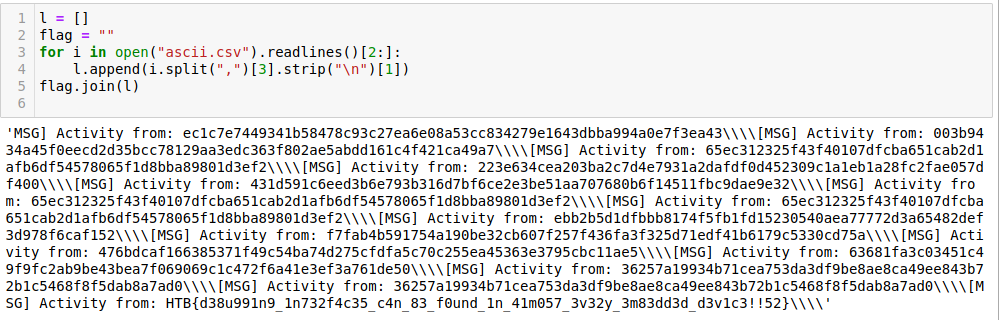
\includegraphics[scale=0.4]{3.1.png}
\end{center}
\subsection{Binary Data Analaysis}


\end{document}
